% This is "sig-alternate.tex" V2.0 May 2012
% This file should be compiled with V2.5 of "sig-alternate.cls" May 2012
%
% This example file demonstrates the use of the 'sig-alternate.cls'
% V2.5 LaTeX2e document class file. It is for those submitting
% articles to ACM Conference Proceedings WHO DO NOT WISH TO
% STRICTLY ADHERE TO THE SIGS (PUBS-BOARD-ENDORSED) STYLE.
% The 'sig-alternate.cls' file will produce a similar-looking,
% albeit, 'tighter' paper resulting in, invariably, fewer pages.
%
% ----------------------------------------------------------------------------------------------------------------
% This .tex file (and associated .cls V2.5) produces:
%       1) The Permission Statement
%       2) The Conference (location) Info information
%       3) The Copyright Line with ACM data
%       4) NO page numbers
%
% as against the acm_proc_article-sp.cls file which
% DOES NOT produce 1) thru' 3) above.
%
% Using 'sig-alternate.cls' you have control, however, from within
% the source .tex file, over both the CopyrightYear
% (defaulted to 200X) and the ACM Copyright Data
% (defaulted to X-XXXXX-XX-X/XX/XX).
% e.g.
% \CopyrightYear{2007} will cause 2007 to appear in the copyright line.
% \crdata{0-12345-67-8/90/12} will cause 0-12345-67-8/90/12 to appear in the copyright line.
%
% ---------------------------------------------------------------------------------------------------------------
% This .tex source is an example which *does* use
% the .bib file (from which the .bbl file % is produced).
% REMEMBER HOWEVER: After having produced the .bbl file,
% and prior to final submission, you *NEED* to 'insert'
% your .bbl file into your source .tex file so as to provide
% ONE 'self-contained' source file.
%
% ================= IF YOU HAVE QUESTIONS =======================
% Questions regarding the SIGS styles, SIGS policies and
% procedures, Conferences etc. should be sent to
% Adrienne Griscti (griscti@acm.org)
%
% Technical questions _only_ to
% Gerald Murray (murray@hq.acm.org)
% ===============================================================
%
% For tracking purposes - this is V2.0 - May 2012

\documentclass{sig-alternate}

\usepackage{graphicx}
\usepackage{enumitem}
\usepackage{rotating}
\usepackage{xcolor}  % color is sufficient
\pdfpagewidth=8.5in
\pdfpageheight=11in
\special{papersize=8.5in,11in}

% Math shortcuts
\newcommand{\xx}{\mathrm{\mathbf{x}}}
\newcommand{\yy}{\mathrm{\mathbf{y}}}
\newcommand{\ttheta}{\mathbf{\theta}}
\newcommand{\eell}{\boldsymbol\ell}


\begin{document}
%
% --- Author Metadata here ---
\conferenceinfo{GECCO'13,} {July 6-10, 2013, Amsterdam, The Netherlands.}
\CopyrightYear{2013}
\crdata{TBA}
\clubpenalty=10000
\widowpenalty = 10000

% --- End of Author Metadata ---

\title{Model Guided Sampling Optimization with Gaussian Processes for Expensive Black-Box Optimization}
%
% You need the command \numberofauthors to handle the 'placement
% and alignment' of the authors beneath the title.
%
% For aesthetic reasons, we recommend 'three authors at a time'
% i.e. three 'name/affiliation blocks' be placed beneath the title.
%
% NOTE: You are NOT restricted in how many 'rows' of
% "name/affiliations" may appear. We just ask that you restrict
% the number of 'columns' to three.
%
% Because of the available 'opening page real-estate'
% we ask you to refrain from putting more than six authors
% (two rows with three columns) beneath the article title.
% More than six makes the first-page appear very cluttered indeed.
%
% Use the \alignauthor commands to handle the names
% and affiliations for an 'aesthetic maximum' of six authors.
% Add names, affiliations, addresses for
% the seventh etc. author(s) as the argument for the
% \additionalauthors command.
% These 'additional authors' will be output/set for you
% without further effort on your part as the last section in
% the body of your article BEFORE References or any Appendices.

\numberofauthors{3} %  in this sample file, there are a *total*
% of EIGHT authors. SIX appear on the 'first-page' (for formatting
% reasons) and the remaining two appear in the \additionalauthors section.
%
\author{
% You can go ahead and credit any number of authors here,
% e.g. one 'row of three' or two rows (consisting of one row of three
% and a second row of one, two or three).
%
% The command \alignauthor (no curly braces needed) should
% precede each author name, affiliation/snail-mail address and
% e-mail address. Additionally, tag each line of
% affiliation/address with \affaddr, and tag the
% e-mail address with \email.
%
% 1st. author
\alignauthor
Lukas Bajer \\
       \affaddr{Faculty of Mathematics and Physics}\\
       \affaddr{Charles University}\\
       \affaddr{Malostranske nam. 25}\\
       \affaddr{Prague 1}\\
       \affaddr{Czech Republic}\\
       \email{bajer@cs.cas.cz}
% 2nd. author
\alignauthor
Viktor Charypar \\
       \affaddr{Faculty of Nuclear Sciences and Physical Engineering}\\
       \affaddr{Czech Technical University in Prague}\\
       \affaddr{Trojanova 13}\\
       \affaddr{120 00 Prague 2}\\
       \affaddr{Czech Republic}\\
       \email{charyvik@fjfi.cvut.cz}
% 3rd. author
\alignauthor
Martin Holena \\
       \affaddr{Institute of Computer Science}\\
       \affaddr{Academy of Sciences of the Czech Republic}\\
       \affaddr{Pod Vodarenskou vezi 2}\\
       \affaddr{182 07 Prague 8}\\
       \affaddr{Czech Republic}\\
       \email{martin@cs.cas.cz}
}

% There's nothing stopping you putting the seventh, eighth, etc.
% author on the opening page (as the 'third row') but we ask,
% for aesthetic reasons that you place these 'additional authors'
% in the \additional authors block, viz.
% Just remember to make sure that the TOTAL number of authors
% is the number that will appear on the first page PLUS the
% number that will appear in the \additionalauthors section.

\maketitle
\begin{abstract}
Model Guided Sampling Optimization (MGSO) is a novel expensive black-box
optimization method based on a combination of ideas from Estimation of 
Distribution Algorithms and global optimization methods using Gaussian 
Processes. The algorithm is described and its implementation tested on 
three benchmark functions as a proof of concept.
\end{abstract}

% Add any ACM category that you feel is needed
\category{G.1.6}{Numerical Analysis}{Optimization}[global optimization,
unconstrained optimization]
\category{F.2.1}{Analysis of Algorithms and Problem Complexity}{Numerical Algorithms and Problems}
\terms{Algorithms}

\keywords{Benchmarking, Black-box optimization, Modeling, Gaussian Processes}

\section{Introduction}

When optimizing expensive objective functions with evolutionary algorithms, the cost of the function 
evaluation dominates the cost of the whole optimization. Our goal is therefore to exploit the knowledge 
of all the previous evaluations. A typical solution in this case is to employ a model based on the evaluated 
candidate solutions. We can then either replace the objective function  with this model for some 
evaluations (a practice known as surrogate modeling) or use the model to guide the selection of candidate 
solutions. We are concerned with the latter.

Estimation of Distribution Algorithms (EDA) present one such approach. An EDA evolves a population of 
candidate solutions in generations, each of which starts with solutions evaluation and selection of the
promising ones. A probabilistic model of the distribution of the better solutions is then built and new 
solutions are sampled from it. A comprehensive overview of EDAs and related methods can be found in \cite{pelikan2006scalable}.

Another approach is using Gaussian Process (GP) model for optimization fitting a GP regression model to the 
data and selecting next candidate solution based on the predictive distribution given by the GP. The most 
promising candidate is added to the dataset and a new model is fitted on the resulting data. A number of candidate 
selection criteria based on predictive distribution were examined by Jones et al. \cite{jones01taxonomy}, 
of which the Probability of Improvement (PoI) is of interest for this work.

We propose a novel optimization method -- Model Guided Sampling Optimization (MGSO) -- based on a combination of 
the GP optimization and EDAs. One can either view the novelty as replacing the distribution model in EDA with 
a probability of improvement of a GP model fitted to all known data, or, from the latter point of view, as, 
instead of maximizing the PoI to find a single candidate solution, sampling a set of candidate solution 
proportionally to the PoI. 

\section{Gaussian process regression}

Gaussian process regression is a stochastic modeling method based on a multidimensional Gaussian distribution. 
GP is a collection of random variables, any finite number of which have a joint Gaussian distribution 
\cite{rasmussen2006gaussian}, realisations of which are functions. We can condition this distribution on training 
data and get a posterior distribution of functions which agree with our observations. A prediction in a testing 
point then gives a Gaussian distribution with some mean and variance. 

A Gaussian process is completely specified by its mean and covariance functions
\begin{align*}
  f(\xx) &\sim \mathcal{GP}\left( m(\xx), k(\xx, \xx')\right) \\
  m(\xx) &= \mathbb{E} \left[ f(\xx) \right] \\
  k(\xx, \xx') &= \mathbb{E} \left[ (f(\xx) - m(\xx))(f(\xx') - m(\xx')) \right] 
\end{align*}

We use a constant mean function and a squared exponential covariance function with
automatic relevance determination
$$
  k_{\mathrm{SE}}(\xx, \xx') = \sigma_f^2 \exp\left( - \frac{1}{2} (\xx - \xx')^\top M (\xx - \xx') \right)
$$
where $ M = \eell^{-2}I $ and fit the hyperparameters $\ttheta = \{ \eell, \sigma_f^2 \}$ by 
maximizing the likelihood $p(\yy | X, \ttheta)$ ($\yy$ are the observations, $X$ is the observation 
points matrix). $\eell$ is a vector of characteristic lengths of the process in each coordinate dimension
and $\sigma_f^2$ is a noise level.

Since the GP gives a Gaussian distribution as prediction, we can think of the distribution's variance
as confidence of the model in it's prediction and use it to guide optimization. Based on both mean 
and variance of the prediction we can easily get a probability of improvement \cite{jones01taxonomy} over a 
certain target $T$ as
$$
 \mathrm{PoI} = \mathrm{\Phi}\left( \frac{T - \bar{f_*}}{\mathbb{V}[f_*]} \right)
$$
where $\Phi$ is the Gaussian cumulative distribution function, $f_*$ is the model prediction (a random
variable), $\bar{f_*}$ is its mean and $\mathbb{V}[f_*]$ is its variance.

MGSO samples this probability of improvement to get a next set of candidate solutions.

\section{The MGSO}

The basic idea of MGSO is similar to global optimization methods by Jones \cite{jones01taxonomy}: Fit a 
GP model to an initial sample of data and let the model predictive distribution guide the optimization. 
The key difference is that MGSO does not maximize the PoI used as a criterion to find a single
solution candidate to evaluate. It rather samples the PoI distribution to get a new population of
candidate solutions. Solutions are then evaluated, the model is fitted to this augmented 
dataset and the process is repeated until one of the stop conditions is met.

To abstract from the search space scaling, MGSO works in an internal, linearly transformed coordinate system 
mapped to $[-1, 1]^D$ and the transformation can be updated during the optimization. Updating it restricts the 
sampling space to a neighborhood of the optimimum, which enables sampling in the situation when the PoI is non-zero 
only in a very small region. Finally, when the neighborhood of the optimum is sufficiently sampled a local search 
is performed to fine tune the optimum. 

\begin{figure}
  \centering
  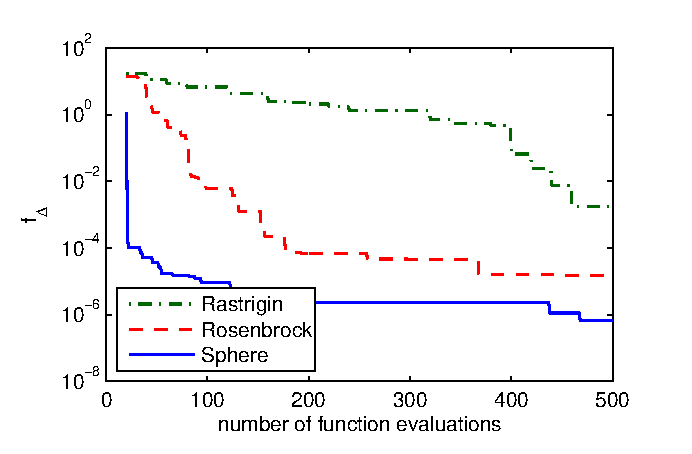
\epsfig{file=mgso_3func_2D.eps,width=7.5cm}

  \caption{
    Median of distances to optimum ($f_{\Delta}$) reached using a number of function evaluations
    for three benchmark functions}
  \label{fig:test}
\end{figure}

Formally, the algorithm performs as follows:
\begin{enumerate}[itemsep=-4pt]
  \item Generate $N_i$ initial samples $\{\xx_0\}$ and evaluate it to get observed values $\{y_0\}$ forming a
    dataset $\mathcal{S}_0 = \{(\xx_0, y_0)\}$.
  \item Until the stop conditions are met for $i = 1, 2, \dots$ repeat steps 3--8
  \item Build a GP model $\mathcal{M}_i$ and fit its hyperparameters $\ttheta$ to the dataset $\mathcal{S}_{i-1}$
  \item Sample $N$ new candidate solutions $\{\xx_i\}$ based on the PoI distribtion of $\mathcal{M}_i$
  \item Evaluate $\{\xx_i\}$ to get ${y_i}$ 
  \item Augment the dataset obtaining $\mathcal{S}_i = \mathcal{S}_{i-1} \cup \{(\xx_i, y_i)\}$
  \item Store the best $(\xx, y) = \underset{y}{\min} \, \mathcal{S}_i$
  \item If rescale conditions are met, restrict the dataset to $\xx \in \times_{i=1}^D [l_i, u_i]$ and
    transform it to $[-1, 1]^D$
  \item Return the best $(\xx, y)$
\end{enumerate}
The bounds $l_i$ and $u_i$ in each coordinate dimension are found as a bounding box of ten nearest samples 
from the current optimum expanded by 10\%. The initial number of samples $N_i$ and population size $N$ are 
input parameters.

Sampling is performed using the Gibbs method \cite{geman1984stochastic} enabling us to sample multivariate 
distributions. In our case we sample candidate solutions from  the empirical distribution propotional to 
the PoI. Samples resulting in ill-con\-di\-tion\-ed covariance matrices of the GP are rejected.

\section{Preliminary results}

As a proof of concept, the method was tested on three benchmark functions from the BBOB toolbox \cite{hansen2012fun} 
in 2D. For each function, 15 optimization runs were performed and best function values 
$f_{\text{best}}$ in each generation were recorded. Figure \ref{fig:test} shows the median of distance to optimum 
$f_{\Delta} = f_{\text{best}} - f_{\text{opt}}$ reached using a given number of function evaluations (limited to 500)
for each benchmark. 

% Figure

%\end{document}  % This is where a 'short' article might terminate

%ACKNOWLEDGMENTS are optional
\section{Acknowledgments}

This work was supported by 
the Grant Agency of the Charles University (GAUK) 278511/2011,
the Grant Agency of the Czech Technical University in Prague, grant No. \\ 
SGS12/196/OHK3/3T/14, 
and the Czech Science Foundation grant (GA\v{C}R) 13-17187S\_9948

%
% The following two commands are all you need in the
% initial runs of your .tex file to
% produce the bibliography for the citations in your paper.
\bibliographystyle{abbrv}
%\bibliography{lb_abstract}  % sigproc.bib is the name of the Bibliography in this case
\begin{thebibliography}{1}

\bibitem{geman1984stochastic}
S.~Geman and D.~Geman.
\newblock Stochastic relaxation, gibbs distributions, and the bayesian
  restoration of images.
\newblock {\em Pattern Analysis and Machine Intelligence, IEEE Transactions
  on}, (6):721--741, 1984.

\bibitem{hansen2012fun}
N.~Hansen, S.~Finck, R.~Ros, and A.~Auger.
\newblock Real-parameter black-box optimization benchmarking 2009: Noiseless
  functions definitions.
\newblock Technical Report RR-6829, INRIA, 2009.
\newblock Updated February 2010.

\bibitem{jones01taxonomy}
D.~Jones.
\newblock A taxonomy of global optimization methods based on response surfaces.
\newblock {\em Journal of Global Optimization}, 21:345--383, 2001.

\bibitem{pelikan2006scalable}
M.~Pelikan and K.~Sastry.
\newblock {\em Scalable optimization via probabilistic modeling: From
  algorithms to applications}, volume~33.
\newblock Springer Verlag, 2006.

\bibitem{rasmussen2006gaussian}
C.~E. Rasmussen.
\newblock Gaussian processes for machine learning.
\newblock 2006.

\end{thebibliography}
% You must have a proper ".bib" file
%  and remember to run:
% latex bibtex latex latex
% to resolve all references
%
% ACM needs 'a single self-contained file'!
%
%APPENDICES are optional
%\balancecolumns
\end{document}
